\chapter{The concept of black hole 3: The global view}
\label{s:glo}

\minitoc

\section{Introduction}

Having attempted in Chaps.~\ref{s:def} and \ref{s:neh} to characterize a black hole by the local
properties of its boundary, we turn now to the general definition of a black
hole. As it could have been anticipated from the naive ``definition'' given
in Sec.~\ref{s:def:first_defin}, the mathematically meaningful definition
of a black hole cannot be local: it has to take into account the full
spacetime structure, in particular its future asymptotics. Indeed, to conclude
firmly that a null geodesic has escaped, one has to wait until the ``end
of time''...

In this chapter, we therefore consider the global spacetime picture to
arrive at the general definition of a black hole in
Sec.~\ref{s:glo:BH}.
This amounts to focusing on the
spacetime asymptotics, which can be seen as
the region where the ``distant observers'' live and may, or may not, receive
light rays from some ``central region''. This far-away structure is best
described in terms of the so-called \emph{conformal completion}, which brings
the spacetime infinity(ies) to a finite distance in another manifold
--- a technique initiated by R.~Penrose\index[pers]{Penrose, R.} \cite{Penro63,Penro64} (see
Refs.~\cite{Fraue04} and \cite{Nicol17} for a review).
We start by investigating the conformal completion of the simplest
spacetime: Minkowski spacetime.

%%%%%%%%%%%%%%%%%%%%%%%%%%%%%%%%%%%%%%%%%%%%%%%%%%%%%%%%%%%%%%%%%%%%%%%%%%%%%%%%%%%%%%%%

\section{Conformal completion of Minkowski spacetime} \label{s:glo:conf_Mink}

In this section $(\M,\w{g})$ is the 4-dimensional Minkowski spacetime,
i.e. $\M$ is a smooth manifold diffeomorphic to $\mathbb{R}^4$ and $\w{g}$
is the metric tensor whose expression in terms of some global coordinates
$(t, x, y, z)$ implementing the diffeomorphism to $\mathbb{R}^4$
(i.e. \emph{Minkowskian coordinates}\index{Minkowskian coordinates})
is
\be \label{e:glo:Mink_metric}
    \w{g} = - \dd t^2 + \dd x^2 + \dd y^2 + \dd z^2 .
\ee

\subsection{Finite-range coordinates on Minkowski spacetime} \label{s:glo:finite_range_Mink}

Since we would like to deal with the ``far'' region, it is natural to introduce
$r := \sqrt{x^2+y^2+z^2}$ and the associated spherical coordinates
$(t,r,\th,\ph)$, which are related to the Minkowskian ones by
\be
    \left\{ \begin{array}{l}
    x = r\sin\th\cos\ph \\
    y = r\sin\th\sin\ph \\
    z = r\cos\th .
    \end{array} \right.
\ee
The coordinates $(t, r,\th,\ph)$ span
$\mathbb{R}\times(0,+\infty)\times (0,\pi) \times (0,2\pi)$; they do not cover
the whole manifold $\M$ as a regular chart (cf. Sec.~\ref{s:bas:def_manif} of Appendix~\ref{s:bas}), but only $\M\setminus \Pi$, where $\Pi$ is the closed half hyperplane defined
by $y=0$ and $x\geq 0$. Once expressed in terms of the
spherical coordinates, the Minkowski metric (\ref{e:glo:Mink_metric}) takes the form
\be \label{e:glo:Mink_metric_spher}
    \w{g} = - \dd t^2 + \dd r^2
        + r^2 \left( \dd\th^2 + \sin^2\th \, \dd\ph^2 \right) .
\ee

\begin{figure}
\centerline{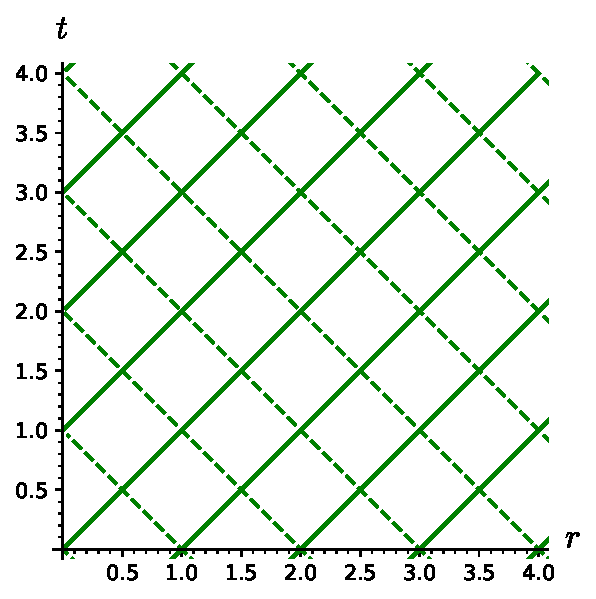
\includegraphics[width=0.5\textwidth]{glo_null_coord.pdf}}
\caption[]{\label{f:glo:null_coord} \footnotesize
Lines of constant null coordinates $u$ (solid) and $v$
(dashed) in terms of the coordinates $(t,r)$.}
\end{figure}


Let us introduce the null coordinate system $(u,v,\th,\ph)$ where $u$ and
$v$ are respectively the retarded\index{retarded!time} and advanced\index{advanced!time}
time defined by (cf. Fig.~\ref{f:glo:null_coord})
\be \label{e:glo:advanced_retarded}
    \left\{ \begin{array}{l}
    u = t - r\\
    v = t + r
    \end{array} \right.
    \iff
    \left\{ \begin{array}{l}
    t = \frac{1}{2} (v+u)\\[1ex]
    r = \frac{1}{2} (v-u) .
    \end{array} \right.
\ee
One has then $\dd u \, \dd v = \dd t^2 - \dd r^2$ and the
metric tensor (\ref{e:glo:Mink_metric_spher}) takes the shape
\be \label{e:glo:Mink_metric_uv}
    \w{g} = - \dd u \, \dd v
        + \frac{1}{4} (v-u)^2 \left(  \dd\th^2 + \sin^2\th \, \dd\ph^2 \right) .
\ee
The coordinates $(u,v)$ span the half part of $\mathbb{R}^2$ defined by
$u<v$. In order to have coordinates within a finite range, let us consider
their arctangents (cf. Fig.~\ref{f:glo:atan}):
\be \label{e:glo:UV_uv}
    \left\{ \begin{array}{l}
    U = \arctan u \\
    V = \arctan v
    \end{array} \right.
    \iff
   \left\{ \begin{array}{l}
    u = \tan U \\
    v = \tan V .
    \end{array} \right.
\ee
Given that $\arctan$ is a monotonically increasing function (cf. Fig.~\ref{f:glo:atan}),
the coordinates $(U,V)$ span the half part of $(-\pi/2, \pi/2)\times (-\pi/2, \pi/2)$
defined by $U < V$:
\be \label{e:glo:span_UV}
    -\frac{\pi}{2} < U < \frac{\pi}{2}, \quad
    -\frac{\pi}{2} < V < \frac{\pi}{2}, \quad\mbox{and}\quad U < V.
\ee

\begin{figure}
\centerline{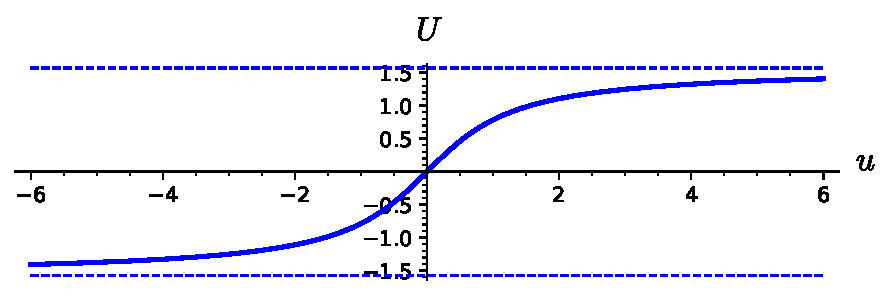
\includegraphics[width=0.8\textwidth]{glo_atan.pdf}}
\caption[]{\label{f:glo:atan} \footnotesize
The arctangent function mapping $\mathbb{R}$ to $(-\pi/2, \pi/2)$.}
\end{figure}

Since
\[
    \D u = \frac{\D U}{\cos^2 U}, \quad \D v = \frac{\D V}{\cos^2 V}
    \quad\mbox{and}\quad
    \tan V - \tan U = \frac{\sin(V-U)}{\cos U \cos V},
\]
the Minkowski metric (\ref{e:glo:Mink_metric_uv})
is expressed in terms of the coordinates $(U,V,\th,\ph)$
as\footnote{See also the SageMath notebook~\ref{s:sam:conformal_Mink}.}
\be \label{e:glo:g_UV}
    \w{g} = \frac{1}{4\cos^2 U \cos^2 V}
    \left[ - 4 \, \dd U \, \dd V + \sin^2(V-U) \left(  \dd\th^2 + \sin^2\th \, \dd\ph^2 \right)
    \right] .
\ee

\begin{remark}
The retarded/advanced times $u$ and $v$ have the dimension of a time, or of a
length in the $c=1$ units that we are using. Therefore, one should introduce
some length scale, $\ell_0$ say, before taking their arctangent and rewrite
(\ref{e:glo:UV_uv}) as
\[
    \left\{ \begin{array}{l}
    U = \arctan (u/\ell_0) \\
    V = \arctan (v/\ell_0)
    \end{array} \right.
    \iff
   \left\{ \begin{array}{l}
    u = \ell_0 \tan U \\
    v = \ell_0 \tan V .
    \end{array} \right.
\]
The coordinates $(U,V)$ are dimensionless and a global factor $\ell_0^2$ should be
introduced in the right-hand side of Eq.~(\ref{e:glo:g_UV}).
However, the length scale $\ell_0$ plays no essential role,
so that, to keep simple notations,
it is omitted in what follows. In other words, we are using units for
which $\ell_0=1$.
\end{remark}

\subsection{Conformal metric} \label{s:glo:conf_metric}

In the right-hand side of (\ref{e:glo:g_UV}),
the terms in square brackets defines a metric
$\w{\tilde{g}}$ such that
\be \label{e:glo:tilde_g_Omega}
    \encadre{ \w{\tilde{g}} = \Omega^2 \w{g} } ,
\ee
where $\Omega$ is the scalar field $\M \rightarrow \mathbb{R}$ obeying
\begin{subequations}
\begin{align}
    \Omega & =  2 \cos U \cos V \label{e:glo:Omega_UV} \\
           & =  \frac{2}{\sqrt{u^2+1}\sqrt{v^2+1}} \label{e:glo:Omega_uv}\\
           & =  \frac{2}{\sqrt{(t-r)^2+1}\sqrt{(t+r)^2+1}} . \label{e:glo:Omega_tr}
\end{align}
\end{subequations}
We notice on (\ref{e:glo:Omega_uv}) and (\ref{e:glo:Omega_tr}) that the function
$\Omega$ never vanishes on $\M$, so that the bilinear form $\w{\tilde{g}}$ defined by
(\ref{e:glo:tilde_g_Omega}) constitutes a well-behaved metric on $\M$.
Moreover, since $\Omega^2 > 0$, $\w{\tilde{g}}$ has the same signature as
$\w{g}$, i.e. $(-,+,+,+)$.
The expression of $\w{\tilde{g}}$ is deduced from (\ref{e:glo:g_UV})
and (\ref{e:glo:Omega_UV}):
\be \label{e:glo:tg_UV}
    \w{\tilde{g}} =  - 4 \, \dd U \, \dd V
        + \sin^2(V-U) \left(  \dd\th^2 + \sin^2\th \, \dd\ph^2 \right) .
\ee

In view of (\ref{e:glo:tilde_g_Omega}), one says that the metric $\w{\tilde{g}}$
is \defin{conformal to}\index{conformal} the metric $\w{g}$, or equivalently,
that the metrics $\w{g}$ and $\w{\tilde{g}}$ are
\defin{conformally related}\index{conformally related metrics},
or that $\w{\tilde{g}}$ arises from $\w{g}$ via a
\defin{conformal transformation}\index{conformal!transformation}.
The scalar field $\Omega$ is called the \defin{conformal factor}\index{conformal!factor}.

A key property of a conformal transformation is to preserve orthogonality
relations, since (\ref{e:glo:tilde_g_Omega}) clearly
implies, at any point $p\in\M$,
\[
    \forall (\w{u},\w{v})\in T_p\M\times T_p\M,\quad
    \w{\tilde{g}}(\w{u},\w{v}) = 0 \iff \w{g}(\w{u},\w{v}) = 0 .
\]
In particular, null vectors for $\w{\tilde{g}}$ coincide with null vectors for $\w{g}$:
\[
    \forall \wl \in T_p\M,\quad
    \w{\tilde{g}}(\wl,\wl) = 0 \iff \w{g}(\wl,\wl) = 0 .
\]
Consequently the light cones of $(\M,\w{g})$ and $(\M,\w{\tilde{g}})$
are identical, which implies that $(\M,\w{g})$ and $(\M,\w{\tilde{g}})$
have the same causal structure.
Moreover, since $\Omega^2>0$, the spacelike and timelike characters of vectors
is preserved as well:
\be
    \begin{array}{ll}
    \forall \w{v} \in T_p\M,\ &
        \w{v} \mbox{\ spacelike for\ } \w{\tilde{g}} \iff \w{v} \mbox{\ spacelike for\ } \w{g} \\
    & \w{v} \mbox{\ timelike for\ } \w{\tilde{g}} \iff \w{v} \mbox{\ timelike for\ } \w{g} .
    \end{array}
\ee
It follows that a curve $\Li$ is timelike (resp. null, spacelike) for $\w{\tilde{g}}$
iff $\Li$ is timelike (resp. null, spacelike) for $\w{g}$. Similarly,
a hypersurface $\Sigma$ is timelike (resp. null, spacelike) for $\w{\tilde{g}}$
iff $\Sigma$ is timelike (resp. null, spacelike) for $\w{g}$.

What about geodesics? Let us first recall that a null curve is not necessarily
a null geodesic (cf. Remark~\ref{r:def:null_curves} on p.~\pageref{r:def:null_curves}
and Appendix~\ref{s:geo}),
so that one cannot deduce from the above results that conformal transformations
preserve null geodesics. However, this turns out to be true:
\begin{prop}[null geodesics preserved by conformal transformations]
Let $\w{g}$ and $\w{\tilde{g}}$ be two Lorentzian metrics on a manifold
$\M$ that are conformally related: $\w{\tilde{g}} = \Omega^2 \w{g}$.
A smooth curve $\Li$ in $\M$ is a null geodesic for $\w{\tilde{g}}$ iff
$\Li$ is a null geodesic for $\w{g}$; any affine parameter $\tilde{\lambda}$
of $\Li$ as a $\w{\tilde{g}}$-geodesic is then related to any affine parameter
$\lambda$ of $\Li$ as a $\w{g}$-geodesic by
\be \label{e:glo:conf_transf_null_geod}
     \derd{\tilde{\lambda}}{\lambda} = a\,  \Omega^2 ,
\ee
where $a$ is a constant.
\end{prop}
\begin{proof}[Sketch of proof]
Write explicitly the geodesic equation [Eq.~(\ref{e:geo:eq_geod})]
and express the Christoffel symbols of $\w{\tilde{g}}$ in terms of those
of $\w{g}$ and the derivatives of $\Omega$ (see e.g. Appendix~D of Wald's
textbook \cite{Wald84} for details).
\end{proof}

On the contrary, conformal transformations preserve neither timelike
geodesics nor spacelike ones.

The coordinates $(U,V)$ are of null type; let us consider instead
the ``time+space'' coordinates $(\tau,\chi)$ defined by\footnote{Notice the
similarity with (\ref{e:glo:advanced_retarded}) up to some $1/2$ factors.}
\be \label{e:glo:tau_chi_U_V}
    \left\{ \begin{array}{l}
    \tau = V + U \\
    \chi = V - U
    \end{array} \right.
    \iff
    \left\{ \begin{array}{l}
    U = \frac{1}{2} (\tau - \chi) \\[1ex]
    V = \frac{1}{2} (\tau + \chi) .
    \end{array} \right.
\ee
Given (\ref{e:glo:span_UV}), the range of these new coordinates is
\be \label{e:glo:range_tau_chi}
    0 < \chi < \pi \quad\mbox{and}\quad
    \chi - \pi < \tau < \pi - \chi .
\ee
In other words, if we draw the Minkowski spacetime in the $(\tau,\chi)$ plane,
it takes the shape of a half-diamond, as depicted in Fig.~\ref{f:glo:conf_diag_Mink}.

\begin{figure}
\centerline{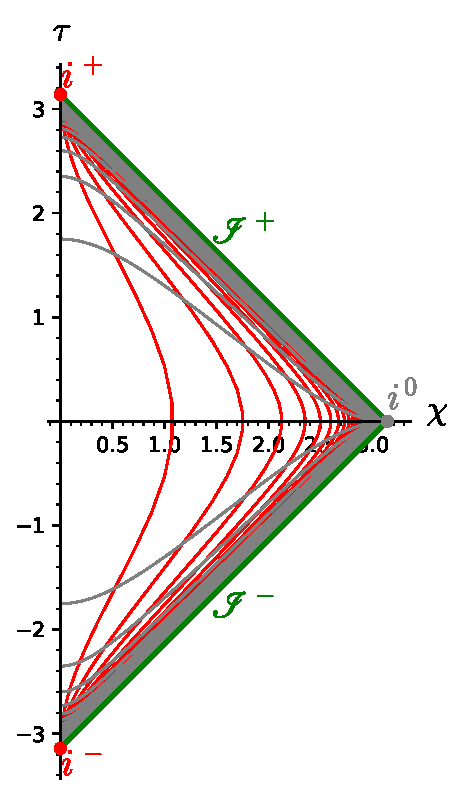
\includegraphics[width=0.35\textwidth]{glo_conf_diag_Mink.pdf}}
\caption[]{\label{f:glo:conf_diag_Mink} \footnotesize
Conformal diagram of Minkowski spacetime. Constant-$r$ curves are drawn in
red, while constant-$t$ ones are drawn in grey.
\textsl{[Figure generated by the notebook \ref{s:sam:conformal_Mink}]}
}
\end{figure}

By combining (\ref{e:glo:advanced_retarded}) (\ref{e:glo:UV_uv}) and
(\ref{e:glo:tau_chi_U_V}), we get the link between $(t,r)$ and
$(\tau,\chi)$:
\be \label{e:glo:tau_chi_t_r}
    \left\{ \begin{array}{l}
    \tau = \arctan(t+r) + \arctan(t-r) \\
    \chi = \arctan(t+r) - \arctan(t-r)
    \end{array} \right.
    \iff
    \left\{ \begin{array}{l}
    \displaystyle t = \frac{\sin\tau}{\cos\tau + \cos\chi}\\[2ex]
    \displaystyle r = \frac{\sin\chi}{\cos\tau + \cos\chi} .
    \end{array} \right.
\ee
We may use these relations to draw the lines $t=\mathrm{const}$ and
$r=\mathrm{const}$ in Fig.~\ref{f:glo:conf_diag_Mink}.

The expression of the conformal factor in the
coordinates $(\tau,\chi,\th,\ph)$ is easily deduced from
(\ref{e:glo:Omega_UV}) and
(\ref{e:glo:tau_chi_U_V}):
\be \label{e:glo:Omega_tau_chi}
    \Omega = \cos\tau + \cos\chi .
\ee


\subsection{Conformal completion} \label{s:glo:conf_complet_Mink}

The expression of the conformal metric in terms of the coordinates
$(\tau,\chi,\th,\ph)$ is easily deduced from that in terms of
$(U,V,\th,\ph)$ as given by (\ref{e:glo:tg_UV}):
\be \label{e:glo:tg_Einstein}
    \w{\tilde{g}} =  - \dd\tau^2
        + \dd \chi^2
        + \sin^2\chi \left(  \dd\th^2 + \sin^2\th \, \dd\ph^2 \right) .
\ee
Restricting to a $\tau = \mathrm{const}$ hypersurface, i.e. setting $\dd\tau=0$,
we recognize the standard metric of the hypersphere
$\mathbb{S}^3$ in the hyperspherical coordinates $(\chi,\th,\ph)$.
Moreover, we notice that the full metric (\ref{e:glo:tg_Einstein})
is perfectly regular even if we relax
the condition on $\tau$ in (\ref{e:glo:range_tau_chi}), i.e. if we
let $\tau$ span the
entire $\mathbb{R}$. We may then consider the manifold
\be
    \mathscr{E} = \mathbb{R}\times \mathbb{S}^3
\ee
and $\w{\tilde{g}}$ as the Lorentzian metric on $\mathscr{E}$ given by
(\ref{e:glo:tg_Einstein}).
The Lorentzian manifold
$(\mathscr{E},\w{\tilde{g}})$ is nothing but the
\defin{Einstein static universe}\index{Einstein!static universe}\index{static!universe (Einstein)}, also called the \defin{Einstein cylinder}\index{Einstein!cylinder}\index{cylinder!Einstein --},
a static solution of the Einstein equation (\ref{e:fra:Einstein_eq})
with $\Lambda > 0$ and some pressureless matter of uniform density
$\rho = \Lambda/(4\pi)$.
We have thus an embedding\footnote{Cf. Sec.~\ref{s:bas:embed} of Appendix~A} of Minkowski spacetime into the Einstein cylinder (cf. Fig.~\ref{f:glo:Einstcyl_Mink}):
\be \label{e:glo:embed_Mink_Einst}
     \Phi:\ \M \longrightarrow \mathscr{E}
\ee
and this embedding is a conformal isometry from
$(\M,\w{g})$ to $(\Phi(\M),\w{\tilde{g}})$.
In the following, we shall identify $\Phi(\M)$ and $\M$, i.e. use the same
symbol $\M$ to denote the subset of $\mathscr{E}$ that is the image of $\M$ via the
embedding (\ref{e:glo:embed_Mink_Einst}).

\begin{figure}
\centerline{\includegraphics[width=0.6\textwidth]{glo_Einstcyl_Mink.pdf}}
\caption[]{\label{f:glo:Einstcyl_Mink}\footnotesize
Two views of the Einstein cylinder $\mathscr{E}$, with the conformal embedding of
Minkowski spacetime $\M$ in it. Each view represents a 2-dimensional cut of $\mathscr{E}$
at $\th=\pi/2$ and $\ph=0$ (one half of the plotted cylinder) or $\ph=\pi$ (the other half).
The $\mathbb{S}^3$ sections of $\mathscr{E}$ are then depicted as horizontal circles,
which are made of two half-circles corresponding to $\ph=0$ and $\ph=\pi$
respectively, with $\chi$ running from $0$ to $\pi$ on both on them.
The plotted piece of $\M$ is then the
2-dimensional cut $(y,z) = (0,0)$ of $\M$, which is a timelike plane spanned
by the coordinates $(t,x)$, with $x\geq 0$ on the $\ph=0$ half cylinder
and $x\leq 0$ on the $\ph=\pi$ half one.
The red curves are the same constant-$r$ curves
as in Fig.~\ref{f:glo:conf_diag_Mink}, while the black curves are
the same constant-$t$ curves as those drawn in grey in Fig.~\ref{f:glo:conf_diag_Mink}.
\textsl{[Figure generated by the notebook \ref{s:sam:conformal_Mink}]}
}
\end{figure}

Since $\mathscr{E}$ and $\M$ have the same dimension, $\M$ is an open subset of $\mathscr{E}$.
Its (topological) closure $\overline{\M}$ in $\mathscr{E}$ is (cf.
Figs.~\ref{f:glo:conf_diag_Mink} and \ref{f:glo:Einstcyl_Mink})
\be
    \overline{\M} = \M \cup \scri^+ \cup \scri^- \cup \left\{ i^0 \right\} \cup
            \left\{ i^+ \right\} \cup \left\{ i^- \right\} ,
\ee
where
\begin{itemize}
\item $\scri^+$ is the hypersurface of $\mathscr{E}$ defined by
$\tau = \pi - \chi$ and $0 < \tau < \pi$ $\iff$
$V=\pi/2$ and $-\pi/2< U < \pi/2$;
\item $\scri^-$ is the hypersurface of $\mathscr{E}$ defined by
$\tau = \chi - \pi $ and $-\pi  < \tau < 0$ $\iff$
$U=-\pi/2$ and $-\pi/2< V < \pi/2$;
\item $i^0$ is the point of $\mathscr{E}$ defined by $\tau=0$ and $\chi=\pi$
$\iff$ $U=-\pi/2$ and $V=\pi/2$;
\item $i^+$ is the point of $\mathscr{E}$ defined by $\tau=\pi$ and $\chi=0$
$\iff$ $U=\pi/2$ and $V=\pi/2$;
\item $i^-$ is the point of $\mathscr{E}$ defined by $\tau=-\pi$ and $\chi=0$
$\iff$ $U=-\pi/2$ and $V=-\pi/2$.
\end{itemize}
It is customary to pronounce $\scri$ as ``scri''\index{scri}, for \emph{script i}.
Note that in the above definitions, we have extended the coordinates $(U,V)$
to $\E$ by the transformations (\ref{e:glo:tau_chi_U_V}); $(U,V,\th,\ph)$
can be then considered as a chart on $\E$ with $(U,V)$ spanning the
infinite strip $0<V-U<\pi$ of $\R^2$ and the metric $\w{\tilde{g}}$ on $\E$
being given by expression (\ref{e:glo:tg_UV}).

\begin{figure}
\centerline{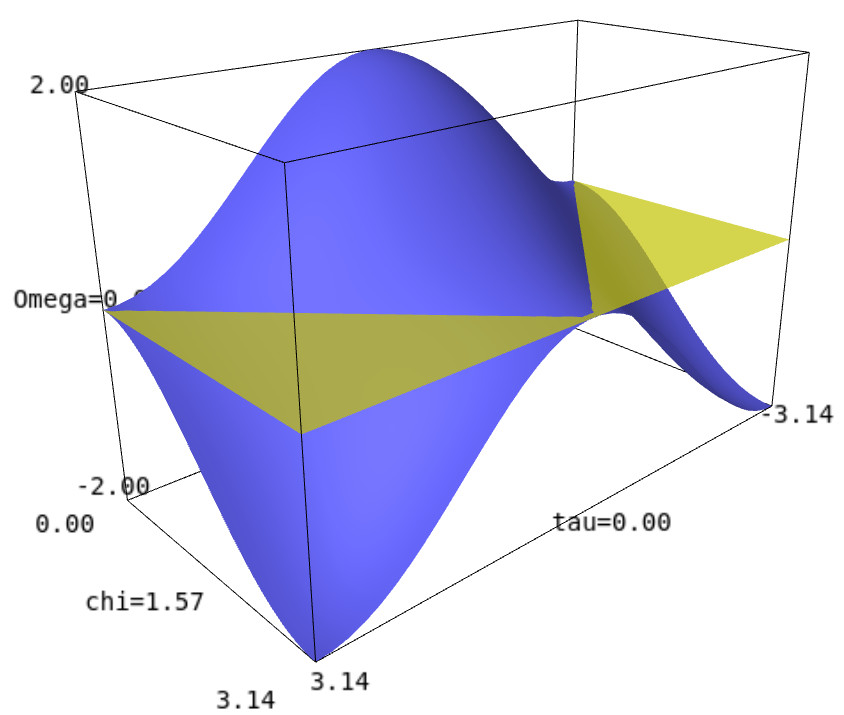
\includegraphics[width=0.45\textwidth]{glo_Omega_Mink.jpg}}
\caption[]{\label{f:glo:Omega_Mink}\footnotesize
Conformal factor $\Omega$ as a function of $(\tau,\chi)$ [cf. Eq.~(\ref{e:glo:Omega_tau_chi})].
Only the part above the yellow horizontal plane ($\Omega=0$) is physical.
\textsl{[Figure generated by the notebook \ref{s:sam:conformal_Mink}]}
}
\end{figure}

\begin{remark}
It is precisely because $\Omega$ vanishes at the
topological boundary of $\M$ in $\E$,
\be
    \overline{\M} \setminus \M = \scri^+ \cup \scri^- \cup \left\{ i^0 \right\} \cup
            \left\{ i^+ \right\} \cup \left\{ i^- \right\} ,
\ee
that the conformal transformation (\ref{e:glo:tilde_g_Omega}) brings the infinity
of Minkowski spacetime to a finite distance (cf. Fig.~\ref{f:glo:Omega_Mink}).
\end{remark}

\begin{remark}
On $\mathbb{S}^3$, the hyperspherical coordinates $(\chi,\th,\ph)$
are singular at $\chi=0$ and $\chi=\pi$, so that setting $\chi=0$ (or $\chi=\pi$)
defines a unique point of $\mathbb{S}^3$, whatever the value of $(\th,\ph)$.
Note also that the vertical left boundary of the diamond drawn in
Fig.~\ref{f:glo:conf_diag_Mink}, i.e. the segment defined by
$\tau\in(-\pi,\pi)$ and $\chi=0$, is \emph{not} a part of the boundary
of $\M$ but merely reflect the coordinate singularity at $\chi=0$, in the same
way that the left vertical boundary of Fig.~\ref{f:glo:null_coord}
is not a boundary of Minkowski spacetime but is
due to the coordinate singularity at $r=0$. Note by the way that
$\chi=0$ implies $r=0$ via (\ref{e:glo:tau_chi_t_r}).
\end{remark}

Let
\be
    \scri := \scri^+ \cup \scri^-
\ee
and
\be \label{e:glo:def_tM_Mink}
    \tilde{\M} := \M \cup \scri .
\ee
$\tilde{\M}$ is naturally a smooth manifold with
boundary\footnote{Cf. Sec.~\ref{s:bas:manif_boundary} for the precise definition.}\index{manifold!with boundary}
and its boundary is $\scri$:
\be
    \partial \tilde{\M} = \scri.
\ee
\begin{remark}
Because the closure $\overline{\M}$ is self-intersecting at the point $i^0$
(cf. Fig.~\ref{f:glo:Einstcyl_Mink}), it is not a manifold with boundary: no open neighborhood of
$i^0$ is homeomorphic to a neighborhood of
$\mathbb{H}^4 = \mathbb{R}^3\times {[0,+\infty)}$,
as the definition of a manifold with boundary would
require, cf. Sec.~\ref{s:bas:manif_boundary}.
At the points $i^+$ and $i^-$, $\overline{\M}$ can be considered as a
topological manifold with boundary, but not as a \emph{smooth} manifold with boundary.
Hence, the three points $i^0$, $i^+$ and $i^-$ are excluded from the definition
of the manifold with boundary $\tilde{\M}$.
\end{remark}

\begin{figure}
\centerline{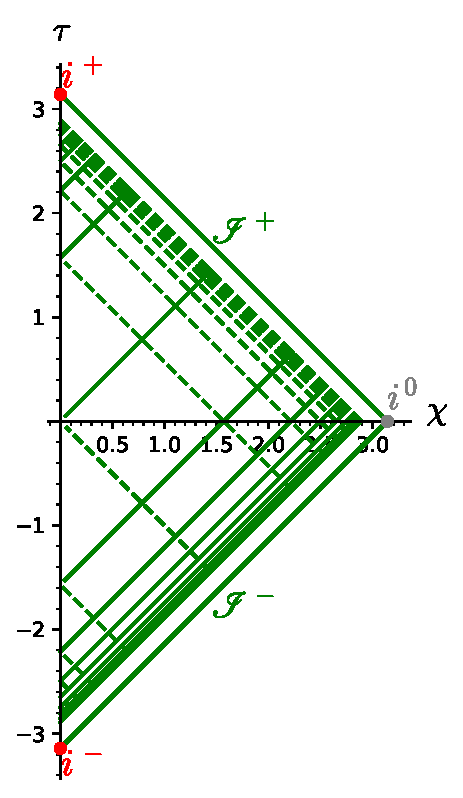
\includegraphics[width=0.35\textwidth]{glo_conf_Mink_null.pdf}}
\caption[]{\label{f:glo:conf_Mink_null}\footnotesize
Null radial geodesics in the conformal diagram of Minkowski spacetime.
The solid green lines are null geodesics $u=\mathrm{const}$ for
17 values of $u$ uniformly spanning $[-8,8]$, while the dashed green lines are
null geodesics $v=\mathrm{const}$ for 17 values of $v$ uniformly spanning $[-8,8]$.
\textsl{[Figure generated by the notebook \ref{s:sam:conformal_Mink}]}
}
\end{figure}


The hypersurface $\scri^+$ is the location of $\tilde{\M}$ where all radial null geodesics
terminate, while $\scri^-$ is the location of $\tilde{\M}$ where all these geodesics originate (cf. Fig.~\ref{f:glo:conf_Mink_null}). For this
reason $\scri^+$ is called the
\defin{future null infinity}\index{future!null infinity}\index{null!infinity}\index{infinity!future null --}
of $(\M,\w{g})$
and $\scri^-$ the \defin{past null infinity}\index{past!null infinity}\index{infinity!past null --}
of $(\M,\w{g})$.
On the other side, any timelike geodesic of $(\M,\w{g})$ originates at $i^-$ and ends at
$i^+$ (cf. Fig.~\ref{f:glo:conf_diag_Mink}), while any spacelike geodesic
of $(\M,\w{g})$ originates at $i^0$ and terminates there
(after having completed a closed path on $\mathbb{S}^3$, cf. Fig.~\ref{f:glo:Einstcyl_Mink}).
The point $i^+$ is then called the
\defin{future timelike infinity}\index{future!timelike infinity}\index{timelike!infinity}\index{infinity!future timelike --}
of $(\M,\w{g})$,
$i^-$ the \defin{past timelike infinity}\index{past!timelike infinity}\index{infinity!past timelike --}
of $(\M,\w{g})$
and $i^0$ the \defin{spacelike infinity}\index{spacelike!infinity}\index{infinity!spacelike --} of $(\M,\w{g})$.

\begin{prop}
\label{p:glo:Mink_scri_null}
$\scri^+$ and $\scri^-$ are null hypersurfaces of $(\tilde{\M},\w{\tilde{g}})$.
\end{prop}
\begin{proof}
Since $\scri^+$ is defined by $V=\pi/2$, a valid coordinate
system on $\scri^+$ is $(U,\th,\ph)$ with $U$ spanning $(-\pi/2, \pi/2)$.
The metric induced by $\w{\tilde{g}}$ on $\scri^+$ is easily obtained by
setting $V=\pi/2$ in Eq.~(\ref{e:glo:tg_UV}):
\be
    \left. \w{\tilde{g}} \right| _{\scri^+} =
    \cos^2 U  \left(  \dd\th^2 + \sin^2\th \, \dd\ph^2 \right) .
\ee
It appears clearly that the signature of this metric is $(0,+,+)$, i.e. it
is degenerate; hence $\scri^+$ is a null hypersurface of
$(\tilde{\M},\w{\tilde{g}})$. Similarly, $\scri^-$ being defined by
$U=-\pi/2$, a valid coordinate
system on $\scri^-$ is $(V,\th,\ph)$ with $V$ spanning $(-\pi/2, \pi/2)$
and the metric induced by $\w{\tilde{g}}$ on $\scri^-$ is obtained by
setting $U=-\pi/2$ in Eq.~(\ref{e:glo:tg_UV}):
\be
    \left. \w{\tilde{g}} \right| _{\scri^-} =
    \cos^2 V  \left(  \dd\th^2 + \sin^2\th \, \dd\ph^2 \right) .
\ee
Again, it is clearly degenerate, so that $\scri^-$ is null hypersurface of
$(\tilde{\M},\w{\tilde{g}})$.
\end{proof}

The null character of $\scri^+$ and $\scri^-$ appears also clearly in
the conformal diagrams of Figs.~\ref{f:glo:conf_diag_Mink}
and \ref{f:glo:conf_Mink_null}, since
$\scri^+$ and $\scri^-$ are straight lines of slope $\pm 1$ in these diagrams.


\begin{hist}
The idea of using a conformal transformation to treat infinity as a boundary
``at a finite distance'' has been put forward by Roger Penrose\index[pers]{Penrose, R.}
in 1963 \cite{Penro63} and expanded in 1964 in the seminal paper \cite{Penro64},
where Penrose constructed the
conformal completion of Minkowski spacetime as a part of the Einstein cylinder.
In particular, Fig.~3 of Ref.~\cite{Penro64} is equivalent to Fig.~\ref{f:glo:Einstcyl_Mink}.
\end{hist}


%%%%%%%%%%%%%%%%%%%%%%%%%%%%%%%%%%%%%%%%%%%%%%%%%%%%%%%%%%%%%%%%%%%%%%%%%%%%%%%%%%%%%%%%

\section{Conformal completions and asymptotic flatness} \label{s:glo:conf_compl}

Having investigated the asymptotic structure of Minkowski spacetime
via a conformal completion, let us use the latter to define spacetimes
that ``look like'' Minkowski spacetime asymptotically.
A first step is the concept of conformal completion.

\subsection{Conformal completion} \label{s:glo:def_conf_compl}

\begin{greybox}
A spacetime $(\M,\w{g})$ admits a
\defin{conformal completion}\index{conformal!completion}
iff there exists a Lorentzian manifold with boundary
$(\tilde{\M},\w{\tilde{g}})$ (cf. Sec.~\ref{s:bas:manif_boundary} for the definition)
equipped with a smooth non-negative scalar field
$\Omega: \tilde{\M} \rightarrow \mathbb{R}^+$
such that
\begin{enumerate}
\item $\tilde{\M} = \M \cup \scri$, with $\scri := \partial \tilde{\M}$
(the manifold boundary\footnote{As stressed in Remark~\ref{r:bas:manifold_boundary}
in Sec.~\ref{s:bas:manif_boundary}, the set $\partial \tilde{\M}$ is
the boundary of $\tilde{\M}$ as a manifold with boundary; it is not the boundary of
$\tilde{\M}$ as a topological space, the latter being $\varnothing$.} of $\tilde{\M})$;
\item on $\M$, $\w{\tilde{g}} = \Omega^2 \w{g}$;
\item on $\scri$, $\Omega=0$;
\item on $\scri$, $\dd \Omega \not= 0$.
\end{enumerate}
$\scri$ is called the \defin{conformal boundary}\index{conformal!boundary}\index{boundary!conformal --}
of $(\M,\w{g})$ within
the conformal completion $(\tilde{\M},\w{\tilde{g}})$.
\end{greybox}
Condition~1 expresses that $\M$ has been endowed with some boundary.
A rigorous formulation of it would be via an embedding $\Phi:\M \rightarrow \tilde{\M}$,
as in Eq.~(\ref{e:glo:embed_Mink_Einst}), so that
$\tilde{\M} = \Phi(\M) \cup \scri$. However, as above, we identify $\Phi(\M)$
with $\M$ and therefore simply write $\tilde{\M} = \M \cup \scri$.
Conditions~2 and 3 express that the boundary of $\M$, which ``lies at an infinite
distance'' with respect to $\w{g}$, has been brought to a
finite distance with respect to $\w{\tilde{g}}$. Indeed, in terms of
length elements [cf. Eq.~(\ref{e:fra:line_element})], condition~2 implies
\[
    \D s^2 = \frac{1}{\Omega^2} \, \D {\tilde s}^2
\]
with $1/\Omega^2 \rightarrow +\infty$ as one approaches $\scri$
(condition~3).
Finally, condition~4 ensures
that $\scri$ is a regular hypersurface of $\tilde{\M}$.
It is of course fulfilled by Minkowski spacetime, as we can check graphically
on Fig.~\ref{f:glo:Omega_Mink}: the graph of $\Omega$ has no horizontal slope
at $\scri$.

\begin{remark}
The statement that $(\tilde{\M},\w{\tilde{g}})$ is a Lorentzian manifold with
boundary implies that $\w{\tilde{g}}$ is smooth everywhere on $\tilde{\M}$,
including at the boundary $\scri$.
\end{remark}

\begin{remark}
The conformal boundary $\scri$ is not part of the physical spacetime
$\M$, but only of the conformal completion $\tilde{\M}$.
\end{remark}

\begin{remark}
One often speaks about
\emph{conformal compactification}\index{conformal!compactification}\index{compactification}
instead of \emph{conformal completion}, but in general $\tilde{\M}$ is not a
compact manifold. For instance, because we omitted the points $i^+$, $i^-$ and $i^0$,
the completion $\tilde{\M}$ of Minkowski spacetime defined by Eq.~(\ref{e:glo:def_tM_Mink})
is not compact.
\end{remark}

\begin{figure}
\centerline{\includegraphics[height=0.4\textheight]{glo_AdS_completion.pdf}}
\caption[]{\label{f:glo:AdS_completion} \footnotesize
Conformal completion of AdS$_{4}$ spacetime, depicted on the Einstein cylinder.
The conformal boundary $\scri$ is shown in yellow, red lines are lines
$\chi=\mathrm{const}$ (uniformly sampled in terms of $\tan\chi = \sinh\rho$),
green curves are radial null geodesics and the purple curve
is a radial timelike geodesic, bouncing back and forth around $\chi=0$.
\textsl{[Figure generated by the notebook \ref{s:sam:AdS}]}
}
\end{figure}

\begin{example}[conformal completion of AdS$_{4}$ spacetime] \label{x:glo:AdS}
The 4-dimensional anti-de Sitter spacetime\index{anti-de Sitter spacetime}
$(\M,\w{g})$
has been introduced in Example~\ref{x:neh:AdS} of Chap.~\ref{s:neh}.
The metric tensor expressed in the conformal coordinates
$(\tau,\chi,\th,\ph)$ is given by Eq.~(\ref{e:neh:metrix_AdS_conformal}):
\be
    \w{g} = \frac{\ell^2}{\cos^2\chi} \left[ - \dd \tau^2
    + \dd \chi^2 + \sin^2\chi \left( \dd\th^2 + \sin^2\th \, \dd\ph^2 \right) \right] ,
\ee
with $\tau\in\R$, $\chi \in (0,\pi/2)$, $\th\in(0,\pi)$ and $\ph\in(0,2\pi)$.
Defining $\Omega := \ell^{-1}\cos\chi$, we notice that
a conformal completion of $(\M,\w{g})$ is $(\tilde{\M},\w{\tilde{g}})$
where (i) $\tilde{\M}$ is the part $\chi \leq \pi/2$ of the Einstein cylinder\footnote{Recall that on the
Einstein cylinder the range of $\chi$ is $(0,\pi)$, cf. Eq.~(\ref{e:glo:range_tau_chi}).}
introduced in Sec.~\ref{s:glo:conf_complet_Mink}
and (ii)  $\w{\tilde{g}}$ is the metric (\ref{e:glo:tg_Einstein}).
The boundary $\scri = \partial\tilde{\M}$ is then the hypersurface $\chi=\pi/2$
of the Einstein cylinder (cf. Fig.~\ref{f:glo:AdS_completion});
$\scri$ is spanned by the coordinates $(\tau,\th,\ph)$
and its topology is that of a 3-dimensional cylinder: $\scri \simeq \mathbb{R}\times\mathbb{S}^2$.
We notice that conditions 3 and 4 of the definition of a conformal completion
are satisfied: $\Omega = \ell^{-1} \cos\chi = 0$ at $\scri$ and
$\dd\Omega = - \ell^{-1} \sin\chi\, \dd\chi = -\ell^{-1} \dd\chi \not = 0 $
at $\scri$.
The metric induced by $\w{\tilde{g}}$ on $\scri$ is obtained by
setting $\chi=\pi/2$ in (\ref{e:glo:tg_Einstein}):
$- \dd \tau^2 + \dd\th^2 + \sin^2\th \, \dd\ph^2$.
This 3-metric is clearly Lorentzian, which shows that $\scri$ is a timelike
hypersurface of $(\tilde{\M},\w{\tilde{g}})$.
\end{example}

The above example shows that $\scri$ is not necessarily a null hypersurface,
as it is for Minkowski spacetime (cf. Sec.~\ref{s:glo:conf_complet_Mink}).
Actually the causal type of $\scri$ is determined by the cosmological
constant, as follows:
\begin{prop}[causal type of $\scri$ and sign of the cosmological constant]
\label{p:glo:type_scri_sign_Lambda}
If the spacetime dimension obeys\footnote{Cf. Remark~\ref{r:fra:Einstein_eq_n_2} in
Sec.~\ref{s:fra:Einstein_eq}.}
$n\geq 3$ and $\w{g}$ is a solution of Einstein equation with
a cosmological constant $\Lambda$ [Eq.~(\ref{e:fra:Einstein_eq})]
and the trace $T$ of the energy-momentum tensor tends to zero in the
vicinity of $\scri$ (i.e. when $\Omega\rightarrow 0$), then
\begin{itemize}
\item $\scri$ is a null hypersurface of $(\tilde{\M},\w{\tilde{g}})$ iff $\Lambda=0$;
\item $\scri$ is a spacelike hypersurface of $(\tilde{\M},\w{\tilde{g}})$ iff $\Lambda>0$;
\item $\scri$ is a timelike hypersurface of $(\tilde{\M},\w{\tilde{g}})$ iff $\Lambda<0$.
\end{itemize}
\end{prop}
\begin{proof}
It follows from $\w{\tilde{g}} = \Omega^2 \w{g}$ that the Ricci scalars $\tilde{R}$
and $R$ of respectively $\w{\tilde{g}}$ and $\w{g}$ are related by\footnote{This relation is
easily established by starting from Eq.~(2.30) of Hawking \& Ellis' textbook~\cite{HawkiE73} or Eq.~(2.19) on p.~645 of Choquet-Bruhat's one~\cite{Choqu09} and inverting the roles of $\w{\tilde{g}}$ and $\w{g}$, thereby substituting
$\Omega^{-1}$ for $\Omega$.}
\be \label{e:glo:tildeR_R}
    \Omega^2 \tilde{R} = R - (n-1) \left( 2 \Omega \, \tilde{g}^{\mu\nu} \tilde{\nabla}_\mu
    \tilde{\nabla}_\nu \Omega - n \, \tilde{g}^{\mu\nu} \partial_\mu \Omega \partial_\nu \Omega
    \right) ,
\ee
where $n = \mathrm{dim}\, \M$ and $\tilde{\nabla}$ stands for the Levi-Civita connection of
$\w{\tilde{g}}$. Using the trace of the Einstein equation (\ref{e:fra:Einstein_eq_n}) to
express $R$, we get
\[
    \Omega^2 \tilde{R} = \frac{2}{n-2}\left( n \Lambda - 8\pi T \right)
     - (n-1) \left( 2 \Omega \, \tilde{g}^{\mu\nu} \tilde{\nabla}_\mu
    \tilde{\nabla}_\nu \Omega - n \, \tilde{g}^{\mu\nu} \partial_\mu \Omega \partial_\nu \Omega
    \right)
\]
This equation is a priori valid in $\M = \tilde{\M}\setminus\scri$ only.
Taking the limit $\Omega\rightarrow 0$ and
assuming that $T\rightarrow 0$ in that limit, we get, by continuity, an identity
on $\scri$:
\be \label{e:glo:normal_scri_square}
\tilde{g}^{\mu\nu} \partial_\mu \Omega \partial_\nu \Omega \stackrel{\scri}{=}
    - \frac{2}{(n-1)(n-2)} \Lambda .
\ee
Since $\scri$ corresponds to a constant value of the scalar field $\Omega$ ($\Omega=0$),
the left-hand side of this equation is nothing but the scalar square
$\w{\tilde{g}}(\w{n},\w{n})$ of the vector $\w{n}$ normal to $\scri$
defined as the dual with respect to $\w{\tilde{g}}$ of the 1-form
$\dd\Omega$: $n^\alpha = \tilde{g}^{\alpha\mu} \partial_\mu \Omega$
(remember that by hypothesis 4 in the definition
of a conformal completion, $\dd\Omega$ is non-vanishing on $\scri$, so that
$\w{n}$  is a valid normal
vector to $\scri$). Equation~(\ref{e:glo:normal_scri_square}) implies
that the sign of $\w{\tilde{g}}(\w{n},\w{n})$ is the opposite of that of $\Lambda$.
Given the link between the causal type of a hypersurface and the causal type of its normal
(cf. Sec.~\ref{s:def:hor_as_null}), this completes the proof.
\end{proof}

The definition of a black hole shall involve a subcategory of conformal completions:

\begin{greybox}
Let $(\M,\w{g})$ be a time-orientable\footnote{Cf. Sec.~\ref{s:fra:time_orientation}.} spacetime admitting a conformal completion $(\tilde{\M},\w{\tilde{g}})$.
One says that $(\tilde{\M},\w{\tilde{g}})$ is a
\defin{conformal completion at null infinity}\index{conformal!completion!at null infinity}
of $(\M,\w{g})$
iff the boundary $\scri := \partial\tilde{\M}$ obeys
\be \label{e:glo:conf_comp_null_inf}
    \scri = \scri^+ \cup \scri^-,
\ee
with $\scri^+$ (resp. $\scri^-$) being never intersected by any past-directed
(resp. future-directed) causal
curve originating in $\M$. Let us recall that a
\defin{causal curve}\index{causal!curve} is
curve whose tangent vectors are nowhere spacelike.
As for Minkowksi spacetime, we shall call $\scri^+$ the
\defin{future null infinity}\index{future!null infinity}\index{null!infinity}\index{infinity!future null --}
and $\scri^-$ the \defin{past null infinity}\index{past!null infinity}\index{infinity!past null --}
of $(\M,\w{g})$.
\end{greybox}

\begin{remark}
The above definition of $\scri^+$ and $\scri^-$ does not impose
that these two objects are null hypersurfaces of $(\tilde{\M},\w{\tilde{g}})$.
This is true for Minkowski spacetime (Property~\ref{p:glo:Mink_scri_null}),
but cannot hold for spacetimes with a
non-zero cosmological constant (Property~\ref{p:glo:type_scri_sign_Lambda}).
In particular, the following
example exhibits spacelike $\scri^+$ and $\scri^-$.
\end{remark}

\begin{example}[Conformal completion of dS$_{4}$ spacetime]
\label{x:glo:dS4}
The 4-dimensional \defin{de Sitter spacetime}\index{de Sitter spacetime} is
$(\M,\w{g})$ with $\M\simeq \mathbb{R}\times\mathbb{S}^3$ and $\w{g}$ is the metric
whose expression in the so-called \emph{global coordinates}
$(t,\chi,\th,\ph)$ is
\be \label{e:glo:dS4}
    \w{g} = \ell^2 \left[ - \dd t^2
    + \cosh^2 t \left(
    \dd \chi^2 + \sin^2\chi \left( \dd\th^2 + \sin^2\th \, \dd \ph^2 \right) \right) \right] ,
\ee
where $\ell$ is a positive constant. Note that $t$ spans $\mathbb{R}$
while $(\chi,\th,\ph)$ are standard polar coordinates on $\mathbb{S}^3$:
$\chi\in(0,\pi)$, $\th\in(0,\pi)$ and $\ph\in(0,2\pi)$.
 The metric (\ref{e:glo:dS4}) is a solution
of the vacuum Einstein equation\index{Einstein!equation!vacuum --}\index{vacuum!Einstein equation} (\ref{e:fra:vac_Einstein_Lambda}) with
the positive cosmological constant $\Lambda = 3/\ell^2$.
Using coordinates $(\tau,\chi,\th,\ph)$ with
$\tau := 2\arctan(\tanh(t/2)) \in (-\pi/2,\pi/2)$, one gets
\be
    \w{g} = \frac{\ell^2}{\cos^2\tau} \left[ - \dd \tau^2
    + \dd \chi^2 + \sin^2\chi \left( \dd\th^2 + \sin^2\th \, \dd\ph^2 \right) \right] .
\ee
Defining $\Omega := \ell^{-1}\cos\tau = (\ell\cosh t)^{-1}$, we notice that
a conformal completion of $(\M,\w{g})$ is $(\tilde{\M},\w{\tilde{g}})$
where (i) $\tilde{\M}$ is the part $-\pi/2\leq \tau \leq \pi/2$ of the Einstein cylinder
introduced in Sec.~\ref{s:glo:conf_complet_Mink}
and (ii)  $\w{\tilde{g}}$ is the metric (\ref{e:glo:tg_Einstein}).
The boundary $\scri = \partial\tilde{\M}$ has two connected components:
$\scri^+$, which is the hypersurface $\tau = \pi/2$ of $\tilde{\M}$, and
$\scri^-$, which is the hypersurface $\tau = -\pi/2$.
Both $\scri^+$ and $\scri^-$ are spanned by the coordinates $(\chi,\th,\ph)$
and their topology is that of $\mathbb{S}^3$.
We notice that conditions 3 and 4 of the definition of a conformal completion
are satisfied: $\Omega = \ell^{-1} \cos\tau = 0$ at $\scri$ and
$\dd\Omega = - \ell^{-1} \sin\tau\, \dd\tau = \pm \ell^{-1} \dd\tau \not = 0 $
at $\scri$.
The metric induced by $\w{\tilde{g}}$ on $\scri$ is obtained by
setting $\tau=\pm\pi/2$ in (\ref{e:glo:tg_Einstein}):
$\dd \chi^2 + \sin^2\chi \left( \dd\th^2 + \sin^2\th \, \dd\ph^2 \right) $.
This 3-metric is clearly Riemannian (this is actually the standard round metric
of $\mathbb{S}^3$), which shows that $\scri$ is a spacelike
hypersurface of $(\tilde{\M},\w{\tilde{g}})$. This of course agrees with
Property~\ref{p:glo:type_scri_sign_Lambda}, given that $\Lambda > 0$.
Finally, it is clear that
any causal curve originating in $\M$ that intersects $\scri^+$ must approach
$\tau=\pi/2$ from below, i.e. cannot be past-directed. Similarly any
causal curve originating in $\M$ that intersects $\scri^-$ must approach
$\tau=-\pi/2$ from above, i.e. cannot be future-directed. We conclude
that $(\tilde{\M},\w{\tilde{g}})$ is a conformal completion at null infinity
of the de Sitter spacetime.
\end{example}

\subsection{Asymptotic flatness} \label{s:glo:asymp_flat}

Penrose\index[pers]{Penrose, R.} \cite{Penro64,Penro68} has defined
a spacetime $(\M,\w{g})$ to be \defin{asymptotically simple}\index{asymptotically!simple} iff there exists
a conformal completion $(\tilde{\M},\w{\tilde{g}})$
of $(\M,\w{g})$
such that every null geodesic in $\M$ has two endpoints in $\scri$.

The last condition, which is verified by Minkowski spacetime (cf. Fig.~\ref{f:glo:conf_Mink_null}),
de Sitter spacetime and anti-de Sitter spacetime (cf. the null geodesics in
Fig.~\ref{f:glo:AdS_completion}), is rather restrictive. In particular, it excludes
black hole spacetimes, since, almost by definition, the latter contain null
geodesics that have no endpoint on $\scri^+$, having only a past endpoint
on $\scri^-$, as far as $\scri$ is concerned. To cope with these spacetimes,
Penrose\index[pers]{Penrose, R.} has also introduced the following definition \cite{Penro68}:
a spacetime $(\M,\w{g})$ is
\defin{weakly asymptotically simple}\index{weakly!asymptotically simple} iff
there exists an open subset $\mathscr{U}$ of $\M$ and
an asymptotically simple spacetime $(\M_0, \w{g}_0)$
with an open neighborhood $\mathscr{U}_0$ of $\scri_0 = \partial \tilde{\M}_0$
in $\tilde{\M}_0$ such that $(\mathscr{U}_0\cap \M_0,\w{g}_0)$ is
isometric to $(\mathscr{U},\w{g})$.

\begin{remark}
For a given weakly asymptotically simple spacetime, there may be different
(non overlapping) regions $\mathscr{U}$ satisfying the above property.
For instance we shall see in Chap.~\ref{s:ker}
that there are an infinite series of them in the (maximally extended) Kerr spacetime.
\end{remark}

Finally one says that a spacetime $(\M,\w{g})$ is
\defin{asymptotically flat}\index{asymptotically!flat}\index{flat!asymptotically --}
(or more precisely \defin{weakly asymptotically simple and empty}\index{weakly!asymptotically simple and empty} \cite{HawkiE73})
iff $(\M,\w{g})$ is weakly asymptotically simple and the Ricci tensor of
$\w{g}$ vanishes in an open neighborhood of $\scri$: $\w{R} = 0$.

\begin{example}
The de Sitter and anti-de Sitter spacetimes are asymptotically simple but
are not asymptotically flat.
\end{example}

Penrose \cite{Penro65b} (see also \cite{Fraue04}) has shown that if $(\M,\w{g})$
is asymptotically simple and empty, the Weyl tensor of $\w{g}$ (cf. Sec.~\ref{s:bas:Weyl})
vanishes at $\scri$. Since the
Ricci tensor is zero, this implies that the full Riemann curvature tensor vanishes
at $\scri$ [cf. Eq.~(\ref{e:bas:Weyl})], hence the qualifier \emph{asymptotically flat}.

The following property holds:
\begin{prop}
The conformal boundary $\scri$ of an asymptotically flat spacetime $(\M,\w{g})$
is a null hypersurface of the conformal completion $(\tilde{\M},\w{\tilde{g}})$.
\end{prop}
\begin{proof}
Consider Eq.~(\ref{e:glo:tildeR_R}). Near $\scri$, we have $R=0$ by the
very definition of asymptotic flatness. The limit $\Omega\rightarrow 0$
results then in
$\tilde{g}^{\mu\nu} \partial_\mu \Omega \partial_\nu \Omega \stackrel{\scri}{=} 0$,
which, following the argument in the proof on p.~\pageref{e:glo:tildeR_R}, implies that
$\scri$ is a null hypersurface.
\end{proof}


%%%%%%%%%%%%%%%%%%%%%%%%%%%%%%%%%%%%%%%%%%%%%%%%%%%%%%%%%%%%%%%%%%%%%%%%%%%%%%%%%%%%%%%%

\section{Black holes} \label{s:glo:BH}

\subsection{Preliminaries regarding causal structure}  \label{s:glo:causal_struct}

Before we proceed to the precise definition of a black hole, let us introduce
some concepts regarding the causal structure of a given time-orientable spacetime $(\M,\w{g})$.
For any subset $S$ of $\M$, one defines
\begin{itemize}
\item the \defin{chronological future of $S$}\index{chronological!future}\index{future!chronological --} as the set $I^+(S)$ of all
points of $\M$ that can be reached from a point of $S$ by a future-directed
timelike curve of nonzero extent;
\item the \defin{causal future of $S$}\index{causal!future}\index{future!causal --} as the set $J^+(S)$ of
all points that either are in $S$ or can be reached from a point of $S$ by a future-directed
causal curve;
\item the \defin{chronological past of $S$}\index{chronological!past}\index{past!chronological --} as the set $I^-(S)$ of all
points of $\M$ that can be reached from a point of $S$ by a past-directed
timelike curve of nonzero extent;
\item the \defin{causal past of $S$}\index{causal!past}\index{past!causal --} as the set $J^-(S)$ of
all points that either are in $S$ or can be reached from a point of $S$ by a past-directed
causal curve.
\end{itemize}
From the above definitions, one has always $S \subset J^\pm(S)$ and
$I^\pm(S) \subset J^\pm(S)$.

\begin{remark}
One has not necessarily $S \subset I^\pm(S)$. For instance,
if $\M$ does not contain
any closed timelike curve, one has  $S \cap I^\pm(S) = \varnothing$ for
$S = \{p\}$ with $p$ being any point of $\M$.
\end{remark}

Here are some basic topological properties of the future and past sets
defined above (see e.g. \S~6.2 of \cite{HawkiE73} or Chap.~14 of
\cite{ONeil83} for proofs):
\begin{itemize}
\item
$I^\pm(S)$ is always an open subset\footnote{This property is a direct
consequence of Lemma~\ref{p:glo:lem1} in Sec.~\ref{s:glo:properties_H} below.} of $\M$, while
$J^\pm(S)$ is not necessarily a closed subset.
\item The interior of $J^\pm(S)$ is $I^\pm(S)$:
\be \label{e:glo:int_JS_IS}
    \mathrm{int}\, J^\pm(S) = I^\pm(S).
\ee
\item Both sets have the same closure:
\be \label{e:glo:clos_JS_IS}
    \overline{J^\pm(S)} = \overline{I^\pm(S)} .
\ee
\item
It follows from (\ref{e:glo:int_JS_IS}) and (\ref{e:glo:clos_JS_IS})
that both sets share the same (topological) boundary:
\be \label{e:glo:boundary_JS_IS}
    \partial J^\pm(S) = \partial I^\pm(S).
\ee
\end{itemize}
The subset of the causal future (resp. past) of $S$ formed by points that cannot be connected
to $S$ by a timelike curve is called the \defin{future horismos}\index{future!horismos}\index{horismos}
(resp. \defin{past horismos}\index{past!horismos})
of $S$ and is denoted by $E^+(S)$ (resp. $E^-(S)$):
\be
    E^+(S) :=  J^+(S) \setminus I^+(S) \qand
    E^-(S) :=  J^-(S) \setminus I^-(S) .
\ee
The horismos $E^\pm(S)$ is formed by null geodesics emanating from points in $S$
(cf. Proposition~4.5.10 of Ref.~\cite{HawkiE73}).
One has $E^\pm(S) \subset \partial J^\pm(S)$.
The spacetime $(\M,\w{g})$
is said to be \defin{causally simple}\index{causally simple}\index{simple!causally --}
iff for every compact set $K\subset \M$, $E^\pm(K) = \partial J^\pm(K)$. This is
equivalent to saying that $J^+(K)$ and $J^-(K)$ are closed subsets of $\M$.

\subsection{General definition of a black hole} \label{s:glo:def_BH}

We are now in position to give the general definition of a black hole.
We shall do it for a spacetime $(\M,\w{g})$ that admits a conformal completion
at null infinity as defined in Sec.~\ref{s:glo:conf_compl} and thus
possesses a future null infinity $\scri^+$.
Moreover, we shall assume that $\scri^+$ is \defin{complete}\index{complete!future null infinity}: if $\scri^+$
is a null hypersurface, which occurs if $(\M,\w{g})$ is asymptotically flat
(cf. Sec.~\ref{s:glo:asymp_flat}),
this means that $\scri^+$ is generated by complete\footnote{Let us recall
that a geodesic is \emph{complete} iff its affine parameters range through the whole of
$\R$, cf. Sec.~\ref{s:geo:existence_uniqueness}
in Appendix~\ref{s:geo}. In particular, such a geodesic is inextendible.}
null geodesics.
The completeness condition is imposed to avoid ``spurious'' black holes,
such as black holes in Minkowski space (cf. Remark~\ref{s:glo:spurious_bh} below).
The neighborhood of $\scri^+$
in $\tilde{\M}$ can then be considered as the infinitely far region
reached by outgoing null geodesics. If a null geodesic does not reach this
region, it can be considered as being trapped somewhere else in spacetime: this
``somewhere else'' constitutes the black hole region.

\begin{greybox}
Let $(\M,\w{g})$ be a spacetime with a conformal completion at null infinity
such that $\scri^+$ is complete;
the \defin{black hole region}\index{black hole!region}
is the set of points of $\M$ that are not in the causal past of the future null
infinity (cf. Fig.~\ref{f:glo:def_bh}):
\be \label{e:glo:def_BH}
    \encadre{\mathscr{B} := \M \setminus (J^-(\scri^+)\cap\M) } .
\ee
If $\mathscr{B} \neq \varnothing$, one says
that the spacetime $(\M,\w{g})$ \defin{contains a black hole}\index{black hole} or that
$(\M,\w{g})$ is a \defin{black hole spacetime}\index{black hole!spacetime}.
\end{greybox}
The black hole region is thus the set of points of $\M$
from which no future-directed causal curve in $\tilde{\M}$ reaches $\scri^+$.


\begin{figure}
\centerline{\includegraphics[width=0.6\textwidth]{glo_def_bh.pdf}}
\caption[]{\label{f:glo:def_bh} \footnotesize
The black hole region $\mathscr{B}$ defined as the complement of
the causal past of the future null infinity, $J^-(\scri^+)$.}
\end{figure}


\begin{example}
The Minkowski spacetime contains no black hole, for all future-directed null geodesics
terminate at $\scri^+$ (cf. Fig.~\ref{f:glo:conf_Mink_null}).
More generally, any asymptotically simple spacetime contains no black hole.
\end{example}

\begin{example}
The prototype of a black hole is the \emph{Schwarzschild black hole}; it will
be shown in Sec.~\ref{s:sch:BH} that the Schwarzschild spacetime contains
a region $\mathscr{B}$ that fulfills the above definition of a black hole.
The corresponding event horizon is nothing but the
Schwarzschild horizon\index{Schwarzschild!horizon} considered in the examples
of Chaps.~\ref{s:def} and \ref{s:neh}.
\end{example}

\begin{remark} \label{s:glo:spurious_bh}
If we release the assumption of $\scri^+$-completeness in the above definition,
we may end up with unphysical or ``spurious'' black holes.
For instance, let us consider the conformal completion of Minkowski spacetime
$(\M,\w{g})$ resulting from its embedding in the Einstein cylinder
$(\E,\w{\tilde{g}})$, as in
Sec.~\ref{s:glo:conf_complet_Mink},
keeping the same $\scri^-$ but
defining $\scri^+$ as the
hypersurface of $\E$ given by $\tau = \pi - \chi$
and $0<\tau<\pi/2$, instead of  $0<\tau<\pi$ in Sec.~\ref{s:glo:conf_complet_Mink}.
The manifold with boundary $\tilde{\M} := \M \cup \scri^+ \cup \scri^-$,
equipped with the Einstein cylinder metric $\w{\tilde g}$, is then a conformal completion
of $(\M,\w{g})$ at null infinity. With such a $\scri^+$, the black hole region
defined by (\ref{e:glo:def_BH}) is non-empty, as shown in Fig.~\ref{f:glo:spurious_bh}.
\end{remark}

\begin{figure}
\centerline{\includegraphics[height=0.3\textheight]{glo_spurious_bh.pdf}}
\caption[]{\label{f:glo:spurious_bh} \footnotesize
Spurious black hole region $\mathscr{B}$ in Minkowski spacetime resulting
from a conformal completion with an incomplete $\scri^+$.
Compare with Fig.~\ref{f:glo:conf_Mink_null}.}
\end{figure}


\begin{remark}
\label{r:glo:HE_BH_def}
Some authors (in particular Hawking and Ellis \cite{HawkiE73}) define a
\emph{black hole} as a connected component of
$\Sigma(\tau) \cap \mathscr{B}$, where $\Sigma(\tau)$ is a spacelike
hypersurface that is a slice of the future development of a partial
Cauchy surface\footnote{The concepts of \emph{partial Cauchy surface}
and \emph{future development} are defined in Sec.~\ref{s:ker:Cauchy_hor}.} $\Sigma(0)$ such that the
closure in $\tilde{\M}$ of the domain of dependence of $\Sigma(0)$ contains $\scri^+$.
According to such a definition, a black hole is a $(n-1)$-dimensional object,
while the black hole region $\mathscr{B}$ defined above is a $n$-dimensional object.
\end{remark}

If $\mathscr{B}\not=\varnothing$, the boundary $\Hor$ of the black hole region
is called the \defin{future event horizon}\index{future!event horizon}
(or simply the \defin{event horizon}\index{event!horizon}
when no ambiguity may arise):
\be
    \encadre{\Hor := \partial \mathscr{B}}.
\ee
By plugging expression (\ref{e:glo:def_BH}) for $\mathscr{B}$ in the standard
identity $\partial \mathscr{B} =
\overline{\mathscr{B}} \cap \overline{\M\setminus \mathscr{B}}$, we get
an equivalent expression for $\Hor$:
\[
    \Hor = \overline{\M \setminus (J^-(\scri^+)\cap\M)} \cap
        \overline{(J^-(\scri^+)\cap\M)}
        = \partial(J^-(\scri^+)\cap\M) .
\]
Now, the boundary of $J^-(\scri^+)$ in $\tilde{\M}$ is
$\partial J^-(\scri^+) = \partial (J^-(\scri^+)\cap\M) \cup \scri^+$, so that
$\partial J^-(\scri^+) \cap \M =  \partial(J^-(\scri^+)\cap\M)$; hence
\be \label{e:glo:Hor_bound_past_scrip}
    \encadre{\Hor = \partial J^-(\scri^+) \cap \M }.
\ee
In words: the future event horizon $\Hor$ is the part of the boundary of the causal past
of the future null infinity $\scri^+$ that lies in $\M$ (cf. Fig.~\ref{f:glo:def_bh}).
Note that thanks to identity (\ref{e:glo:boundary_JS_IS}), we can write as
well
\be
    \Hor = \partial I^-(\scri^+) \cap \M .
\ee

\subsubsection{White hole}

By inverting past and future in the black hole definition (\ref{e:glo:def_BH}), one defines
the \defin{white hole region}\index{white hole} of a
spacetime $(\M,\w{g})$ with a conformal completion at null infinity as the
complement within $\M$ of the causal future of the past null infinity $\scri^-$:
\be \label{e:glo:def_white_hole}
    \encadre{\mathscr{W} := \M \setminus (J^+(\scri^-)\cap \M) } .
\ee
The white hole region is thus the set of points of $\M$
from which no past-directed causal curve in $\tilde{\M}$ reaches $\scri^-$.
The boundary of white hole region is called the
\defin{past event horizon}\index{past!event horizon}:
\be
    \encadre{\Hor^- := \partial \mathscr{W} = \partial J^+(\scri^-) \cap \M } .
\ee

\begin{remark}
The name \defin{white fountain}\index{white!fountain} is sometimes used
instead of \emph{white hole}. Actually, this name may seem better suited
to describe the time symmetric of a black hole: one can fall into a hole, while
one is expelled by a fountain.
\end{remark}

\begin{example}
We shall encounter an example of white hole in the maximal extension of
Schwarzschild spacetime, to be discussed in Chap.~\ref{s:max} (cf. Sec.~\ref{s:max:black_white}).
\end{example}

The \defin{domain of outer communications}\index{domain of outer communications}
is the part $\langle\langle \M\rangle\rangle$ of $\M$ that lies neither
in the black hole region nor in the white hole one:
\be \label{e:glo:def_doc}
    \langle\langle \M\rangle\rangle := \M\setminus (\mathscr{B}\cup \mathscr{W} )
            = \left( J^-(\scri^+) \cap J^+(\scri^-) \right) \cap \M .
\ee
The last equality, which is a direct consequence of the definitions of
$\mathscr{B}$ and $\mathscr{W}$, shows that the domain of outer communications
is the set of points from which it is possible to send a signal to and to
receive a signal from arbitrarily far regions.
It also follows immediately from the definitions of the two event horizons
that the boundary of the domain of outer communications is their union:
\be
    \partial \langle\langle \M\rangle\rangle  = \Hor \cup \Hor^- .
\ee

\begin{hist} \label{h:glo:black_hole_name}
The term \emph{event horizon} has been introduced by Wolfgang Rindler\index[pers]{Rindler, W.} in 1956 \cite{Rindl56}
in the context of a single observer moving in some cosmological spacetime.
Regarding the name \emph{black hole}, the standard
story is that it has been coined by John~A.~Wheeler\index[pers]{Wheeler, J.A.} in the end of 1967,
following a suggestion shouted from the audience during one of his conference.
However, a recent study \cite{HerdeL18} reveals that the expression \emph{black hole}
circulated as early as 1963 in the first Texas Symposium on Relativistic Astrophysics
held in Dallas,
while discussing the discovery of quasars, and could have been forged by
Robert Dicke\index[pers]{Dicke, R.} in some lecture given in 1961.
The term \emph{black hole} rapidly superseded the previous names
\emph{frozen star}\index{frozen star}, \emph{collapsed star}, or \emph{astre occlus}
(the latter still appearing along \emph{black holes} in the title of
the proceedings of the famous Les Houches summer school of 1972 \cite{DeWit73}).
For instance, \emph{``black hole''} was used abundantly, albeit with
quotes, in a review article by Roger Penrose\index[pers]{Penrose, R.} published
in 1969 \cite{Penro69}. In the same article, Penrose defined the \emph{absolute event horizon}
as $\partial J^-(\scri^+)$ (actually $\partial I^-(\scri^+)$, but both coincide, cf.
Eq.~(\ref{e:glo:boundary_JS_IS})), i.e. essentially the identity (\ref{e:glo:Hor_bound_past_scrip}), but he did not provide any formal definition of the
black hole region as $ \M \setminus (J^-(\scri^+)\cap\M)$ [Eq.~(\ref{e:glo:def_BH})].
It seems that the latter appears first in an ``instant-of-time'' version
(cf. Remark~\ref{r:glo:HE_BH_def}) in a famous article by Stephen Hawking\index[pers]{Hawking, S.W.} published in 1972 \cite{Hawki72}.
The expression \emph{domain of outer communications} has been introduced in 1971 by
Brandon Carter\index[pers]{Carter, B.} \cite{Carte71}.
\end{hist}


\subsection{Properties of the future event horizon} \label{s:glo:properties_H}

Having defined a black hole region in full generality, let us derive the
main properties of its boundary --- the future event horizon $\Hor$.


\begin{prop}[the event horizon as an achronal set]
\label{p:glo:prop1}
A black hole event horizon $\Hor$ is an \defin{achronal set}\index{achronal!set}, i.e. no pair of points of $\Hor$ can be connected
by a timelike curve of $\M$.
\end{prop}

\begin{figure}
\centerline{\includegraphics[height=0.3\textheight]{glo_timelike_stab.pdf}}
\caption[]{\label{f:glo:timelike_stab} \footnotesize
Lemma~\ref{p:glo:lem1}: moving slightly the ends $p$ and $q$ of a timelike curve $\Li$
necessarily results in another timelike curve $\Li'$.}
\end{figure}

Note that in the definition of an achronal set, it is not demanded that the timelike
curve lies entirely in the set (for instance, the set can be discrete, so that no curve
whatsoever lies in it). Accordingly,
an equivalent statement of Property~\ref{p:glo:prop1} is: no timelike curve of $\M$
encounters $\Hor$ at more than one point.

The proof of Property~\ref{p:glo:prop1} relies on the following lemma:
\begin{lemma}[stability of timelike curves with respect to their ends]
\label{p:glo:lem1}
One can ``move the ends'' of any timelike curve
``a little bit'' and still get a timelike curve. More precisely,
if two points $p,q\in\M$ are connected by a timelike curve,
there exists
a neighborhood $U$ of $p$ and a neighborhood $V$ of $q$ such that
any point $p'\in U$ can be connected to any point $q'\in V$ by a timelike curve.
\end{lemma}
\begin{proof}
This is more or less evident on a spacetime diagram (cf. Fig.~\ref{f:glo:timelike_stab})
and a formal proof
can be found as Lemma~3 in Chap.~14 of O'Neill's textbook \cite{ONeil83}.
\end{proof}

\begin{proof}[Proof of Property~\ref{p:glo:prop1}]
Let us assume the negation of Property~\ref{p:glo:prop1}, i.e. that there exists two points
$p$ and $q$
in $\Hor$ that are connected by a timelike curve $\Li$, with $q$
lying in the future of $p$ (cf. Fig.~\ref{f:glo:achronal}).
Invoking Lemma~\ref{p:glo:lem1}, let $U$ and $V$ be the neighborhoods of respectively
$p$ and $q$ within which one can deform $\Li$ to a timelike curve.
Let us choose $p'\in U\cap\mathscr{B}$ ($\mathscr{B}$ being the black hole region)
and $q'\in V\cap J^-(\scri^+)$. Such a choice is
always possible since $p$ and $q$ lie on the boundary between $\mathscr{B}$
and $J^-(\scri^+)$ (cf. Fig.~\ref{f:glo:achronal}).
Since $q'\in J^-(\scri^+)$, the timelike curve linking $p'$ and $q'$ can then be extended to the future in a causal curve $\Li'$ reaching $\scri^+$. This implies $p'\in J^-(\scri^+)$,
which contradicts $p'\in\mathscr{B}$.
\end{proof}

\begin{figure}
\centerline{\includegraphics[width=0.55\textwidth]{glo_achronal.pdf}}
\caption[]{\label{f:glo:achronal} \footnotesize
Proving that $\Hor$ is achronal.}
\end{figure}


\begin{prop}[the event horizon as manifold of codimension 1]
\label{p:glo:prop2}
$\Hor$ is a topological manifold of dimension $n-1$, $n$ being the spacetime
dimension.
\end{prop}

\begin{figure}
\centerline{\includegraphics[width=0.45\textwidth]{glo_hor_manifold.pdf}}
\caption[]{\label{f:glo:hor_manifold} \footnotesize
Proving that $\Hor$ is a topological manifold of dimension $n-1$.}
\end{figure}

\begin{proof}
Let $p\in\Hor$ and $U$ some open neighborhood of $p$ where one can define
a normal coordinate system $(x^\alpha)$. We have then $\wpar_0$ timelike,
$\wpar_i$ spacelike for $i\in\{1,\ldots,n-1\}$ and $\w{g}(\wpar_0, \wpar_i) = 0$.
Let us consider a curve in $U$ defined by $x^1 = a_1$,..., $x^{n-1} = a_{n-1}$,
where $a_1$, ..., $a_{n-1}$ are $n-1$ constants.
This curve is timelike, since it has $\wpar_0$ as a tangent vector
(cf. Fig.~\ref{f:glo:hor_manifold}).
It therefore intersects $\Hor$ at a single point $q$, for $\Hor$ is achronal
(Property~\ref{p:glo:prop1}).
Let us then give the coordinates $(y^i) = (a_1,\ldots,a_{n-1})$ to $q$.
By varying $(a_1,\ldots,a_{n-1})$, we get a homeomorphism from $U\cap\Hor$
to an open subset of $\mathbb{R}^{n-1}$.
\end{proof}

\begin{remark}
Generically, the topological manifold $\Hor$ is not a smooth manifold, for it
contains some points (the crossovers defined below) at which it is not differentiable.
Actually $\Hor$ is slightly more than a mere topological submanifold of $\M$: it is a
\emph{Lipschitz submanifold} of $\M$. The latter is
intermediate between a topological submanifold, i.e.
a submanifold of class $C^0$ (continuous), and a differentiable submanifold of
class $C^1$. On $U\cap\Hor$, the function $x^0$ is a Lipschitz function
of the coordinates $(y^i)$: $\left|x^0(y^i) - x^0({y'}^i)\right| < K \sqrt{\sum_i (y^i - {y'}^i)^2}$.
This follows from the achronal character of $\Hor$: the points of coordinates
$(y^i)$ and $({y'}^i)$ cannot have a too large separation in terms of $x^0$,
otherwise they would be timelike separated.
Hence, one says that $\Hor$ is a \defin{Lipschitz submanifold}\index{Lipschitz submanifold} of $\M$. The notation $C^{1-}$ (i.e. a kind of intermediate between
$C^0$ and $C^1$) is generally used to denote Lipschitz submanifolds.
\end{remark}

\begin{prop}[the event horizon ruled by never leaving null geodesics \textnormal{(Penrose\index[pers]{Penrose, R.} 1968 \cite{Penro68})}]
\label{p:glo:prop3}
A black hole event horizon $\Hor$ is ruled by a family of null geodesics,
called the \defin{generators of}\index{generator!of an event horizon} $\Hor$,
 that (i) either lie entirely
in $\Hor$ or never leave $\Hor$ when followed into the future from the
point where they enter $\Hor$, and
(ii) have no endpoint in the future.
Moreover, there is exactly one generator through each point of $\Hor$,
except at special points where null geodesics enter $\Hor$, which are
called \defin{crossovers}\index{crossover point}. A special case
of crossover, called \defin{caustic}\index{caustic}, is a point
where neighboring null geodesics focus and converge while arriving in $\Hor$.
\end{prop}
In particular, once a null geodesic has
merged with $\Hor$ (at a point where it may intersect other null geodesics),
it will stay forever on $\Hor$ and will never intersect any other generator.
The set of all crossovers is called the \defin{crease set}\index{crease set}
\cite{Siino98a,Siino98b,Brill14}.

\begin{figure}
\centerline{\includegraphics[width=0.3\textwidth]{glo_timelike_arc.pdf}}
\caption[]{\label{f:glo:timelike_arc} \footnotesize
Lemma~\ref{p:glo:lem2}: A \emph{causal} curve $\Li$ containing a timelike segment (between
$a$ and $b$ on the figure) can be deformed into a \emph{timelike} curve $\Li'$
with the ends kept fixed (dashed curve).}
\end{figure}

The following proof of Property~\ref{p:glo:prop3}
is adapted from that given in Box~34.1 of MTW \cite{MisneTW73}.
In addition of Lemma~\ref{p:glo:lem1}, it relies on the following lemma.

\begin{lemma}
\label{p:glo:lem2}
Let $\Li$ be a causal curve connecting two points $p$ and $q$
of $\M$. If $\Li$ contains a timelike segment, then there exists an
entirely timelike curve connecting $p$ and $q$.
\end{lemma}
\begin{proof}
We shall only provide a graphical ``proof'', based on the spacetime diagram
of Fig.~\ref{f:glo:timelike_arc}. The causal curve $\Li$ may have parts where it is null (segments $pa$ and $bq$ in Fig.~\ref{f:glo:timelike_arc}); these parts are drawn with
an angle of incline $\theta = \pm 45^\circ$.
If $\Li$ contains a timelike segment (such as $ab$ in Fig.~\ref{f:glo:timelike_arc}), i.e. a segment with $|\theta|>45^\circ$,
it can be deformed, while keeping the same ends, to a curve with $|\theta|>45^\circ$
everywhere, i.e. to a timelike curve.
\end{proof}

\begin{figure}
\centerline{\includegraphics[width=0.55\textwidth]{glo_point_sequence.pdf}}
\caption[]{\label{f:glo:point_sequence} \footnotesize
Causal curve $\Li$ connecting $p$ to $q$ obtained as a limit of causal curves
in $J^-(\scri^+)$.}
\end{figure}

\begin{proof}[Proof of Property~\ref{p:glo:prop3}]
Let $p\in\Hor$ and let $U$ be some convex normal neighborhood\footnote{Basically,
a convex normal neighborhood is an open subset $U$ such that any two points of $U$
can be connected by a geodesic lying entirely in $U$, cf. Sec.~\ref{s:geo:normal_coord}.
There always exists a convex normal neighborhood around any point of a pseudo-Riemannian manifold
(cf. Proposition~7 p.~130 in O'Neill's textbook~\cite{ONeil83}).}
of $p$. Since $p$ lies in the boundary of $J^-(\scri^+)$, it is always possible to
consider
a sequence of points $(p_n)_{n\in\mathbb{N}}$ converging toward $p$
and such that $\forall n\in\mathbb{N},\ p_n \in U \cap J^-(\scri^+)$
(cf. Fig.~\ref{f:glo:point_sequence}).
Since $p_n\in J^-(\scri^+)$,
there exists a future-directed causal curve $\Li_{n}$ from $p_n$ to $\scri^+$
for each $n\in\mathbb{N}$.
The neighborhood $U$ being convex, each $\Li_n$ intersects its boundary $\partial U$
at a unique point, $q_n$ say, in the future of $p_n$: $\{q_n\}=\Li_n \cap \partial U$
(cf. Fig.~\ref{f:glo:point_sequence}).
Since $\partial U$
is compact, the sequence $(q_n)_{n\in\mathbb{N}}$ admits a subsequence,
$(q_{f(n)})_{n\in\mathbb{N}}$ say ($f$ being an increasing
function $\mathbb{N}\rightarrow\mathbb{N}$),
that converges to some limit point $q$.
Since from any point $p_{f(n)}$ arbitrarily close to $p$, there is
the causal curve $\Li_{f(n)}$ to the point $q_{f(n)}$ arbitrarily close to $q$,
one can show that
there exists a future-directed causal curve $\Li$ connecting $p$ to $q$
(cf. Fig.~\ref{f:glo:point_sequence}; see e.g.
Lemma~6.2.1 of Hawking \& Ellis' textbook \cite{HawkiE73}
for a precise demonstration).

As the limit of points in $J^-(\scri^+)$, $q$ lies in the closure
$\overline{J^-(\scri^+)} = J^-(\scri^+) \cup \Hor$, $\Hor$
being the boundary of $J^-(\scri^+)$.
Let us show by contradiction that actually $q\in\Hor$.
If we assume $q\not\in\Hor$, then necessarily $q\in J^-(\scri^+)$.
There exists then an open neighborhood $V$ of $q$ such that $V \subset  J^-(\scri^+)$
(cf. Fig.~\ref{f:glo:q_in_H}).
Let us choose $q'\in V$ such that $q$ is connected to $q'$ via a timelike curve.
We may then extend $\Li$ to a causal curve $\tilde{\Li}$ from $p$ to $\scri^+$
via $q$ and $q'$ (cf. Fig.~\ref{f:glo:q_in_H}). Since $\tilde{\Li}$ contains a timelike segment
(between $q$ and $q'$), we may invoke Lemma~\ref{p:glo:lem2} to deform it into
a timelike curve $\tilde{\Li}'$ between $p$ and $\scri^+$. Then, by Lemma~\ref{p:glo:lem1},
one can ``move the past end'' of $\tilde{\Li}'$
to get a new timelike curve $\tilde{\Li}''$ linking an event $p'\in\mathscr{B}$ close
to $p$ to $\scri^+$ (dotted curve in Fig.~\ref{f:glo:q_in_H}), which is impossible by the very definition of the black hole
region $\mathscr{B}$. Hence $q\in\Hor$.

\begin{figure}
\centerline{\includegraphics[width=0.55\textwidth]{glo_q_in_H.pdf}}
\caption[]{\label{f:glo:q_in_H} \footnotesize
Proving by contradiction that $q$ lies in $\Hor$.}
\end{figure}


The causal curve $\Li$ connecting $p$ to $q$ cannot be timelike since
$p$ and $q$ are both in $\Hor$, which is achronal (Property~\ref{p:glo:prop1}).
Actually, $\Li$ cannot even contain a timelike segment: if it would, then
by Lemma~\ref{p:glo:lem2}, it could
be deformed into a timelike curve between $p$ and $q$, which again would
contradict the achronal character of $\Hor$. Hence $\Li$ is necessarily a null
curve. Moreover, it is a geodesic. Indeed, let us assume it is not.
There is then some non-geodesic null segment of $\Li$, $ab$ say. Now, as shown in Sec.~\ref{s:geo:all_geod} of Appendix~\ref{s:geo},
a curve from $a$ to $b$ is a geodesic iff any of its parametrizations
$P: [\lambda_a,\lambda_b] \rightarrow \M$, $\lambda \mapsto P(\lambda)\in\Li$
is a stationary point of the action
\[
    E_{(a,b)}(P) := \int_{\lambda_a}^{\lambda_b}
        \w{g}(\w{v}, \w{v})  \, \D\lambda ,
\]
where $\w{v} = \D\w{x}/\D\lambda$ is the tangent vector
associated with $P$. For the null segment $ab$ of $\Li$, we have
$E_{(a,b)}(P)=0$. Since $ab$ is assumed to be not geodesic, it is not a
stationary point of $E_{(a,b)}(P)$, which
implies that there exists a nearby curve from $a$ to $b$ with $E_{(a,b)}(P)<0$,
i.e. there exists a curve from $a$ to $b$ with some timelike part.
It follows that $p$ and $q$ can be connected
by a causal curve with a timelike segment. But this feature has been
excluded above. We conclude that $\Li$ is a null geodesic.

At this stage, we have shown that given $p\in\Hor$, there exists
a future-directed null geodesic $\Li$ connecting $p$ to another point $q\in\Hor$.
There remains to show that $\Li$ lies entirely in $\Hor$.
Let us start by showing that $\Li\subset \overline{J^-(\scri^+)}$.
Let $a$ be a generic point of $\Li$ between $p$ and $q$. Since $\Li$ is
null, there exists a point
$a'$ arbitrarily close to $a$ such that $a'$ is connected to $q$ by a
future-directed timelike curve (cf. Fig.~\ref{f:glo:L_in_H}). Thanks to Lemma~\ref{p:glo:lem1}
and the property $q\in \overline{J^-(\scri^+)}$, we may
find a point $q'\in J^-(\scri^+)$ close to $q$ such that $a'$ is connected
to $q'$ by a future-directed timelike curve.
Since $q'\in J^-(\scri^+)$, such a curve can be extended
to a causal curve to $\scri^+$  (the dashed curve
in Fig.~\ref{f:glo:L_in_H}); hence
$a'\in  J^-(\scri^+)$. Since $a'$ is arbitrarily close to $a$, we conclude
that $a\in\overline{J^-(\scri^+)}$.
Then, by repeating the same reasoning as that employed above for proving
$q\in\Hor$, simply replacing $q$ by $a$, we get that $a\in\Hor$. Since
$a$ is a generic point of $\Li$, we conclude that
$\Li$ lies entirely in $\Hor$.

\begin{figure}
\centerline{\includegraphics[width=0.45\textwidth]{glo_L_in_H.pdf}}
\caption[]{\label{f:glo:L_in_H} \footnotesize
Proving that $\Li$ lies entirely in $\Hor$.}
\end{figure}



Given a point $p\in\Hor$, we have thus constructed a
future-directed null geodesic $\Li$ lying entirely in $\Hor$ and
connecting $p$ to another point $q\in\Hor$. One can
repeat the construction
from the point $q$ to get another future-directed null geodesic $\Li'\subset\Hor$
connecting $q$ to another point $q'\in\Hor$. Now $\Li$ and $\Li'$ must
be two segments of the same null geodesic $\Li\cup\Li'$ by the following lemma.
\begin{lemma}
\label{p:glo:lem3}
Let $q\in\Hor$. If $\Li\subset\Hor$ is a null geodesic having $q$ as future end point
and $\Li'\subset\Hor$ is a null geodesic having $q$ as past end point, then
$\Li$ and $\Li'$ have collinear tangent vectors at their common point $q$.
It follows that $\Li$ and $\Li'$ are two segments of a same null geodesic through $q$.
\end{lemma}
\begin{figure}
\centerline{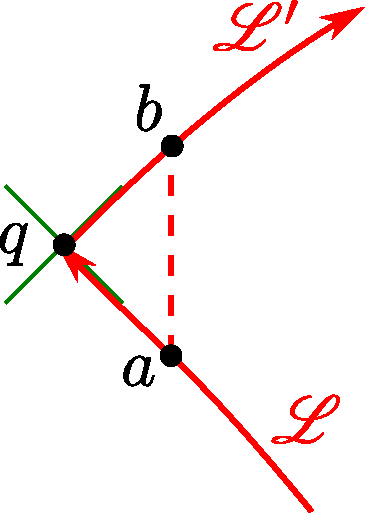
\includegraphics[width=0.17\textwidth]{glo_unique_geod.pdf}}
\caption[]{\label{f:glo:unique_geod} \footnotesize
Proof of Lemma~\ref{p:glo:lem3}.}
\end{figure}
\begin{proof}[Proof of Lemma~\ref{p:glo:lem3}]
Assume that $\Li$ and $\Li'$ have non-collinear tangent vectors at $q$. Then, in
the vicinity of $q$, one can find a point $a\in\Li$ and a point $b\in\Li'$
such that $a$ and $b$ can be connected by a timelike curve (cf.
Fig.~\ref{f:glo:unique_geod}). Since $\Li\subset\Hor$ and $\Li'\subset\Hor$, we have $a\in\Hor$ and
$b\in\Hor$ and therefore we get a contradiction with $\Hor$ being achronal.
\end{proof}
Thanks to Lemma~\ref{p:glo:lem3}, we conclude that $\Li'$ extends $\Li$ to the null geodesic
$\Li\cup\Li'$ entirely lying in $\Hor$. By iterating, we conclude that
the null geodesic $\Li$ through $p$ can be extended indefinitely into the
future. Moreover, it can never leave $\Hor$. Indeed, if $\Li$ would leave $\Hor$ at
some point $q$, by the same procedure used above for $p$, one could construct a future-directed null geodesic
$\Li'\subset\Hor$ starting from $q$; then Lemma~\ref{p:glo:lem3} would imply that
$\Li$ and $\Li'$ would have the same tangent at $q$, which is not compatible
with $\Li$ leaving $\Hor$ at $q$.

Another direct consequence of Lemma~\ref{p:glo:lem3} is that no two distinct null generators
may intersect at a point $p\in\Hor$, except if their segments in the past of
$p$ lie outside $\Hor$.
This completes the proof of Property~\ref{p:glo:prop3}.
\end{proof}


\begin{figure}
\centerline{\includegraphics[width=0.5\textwidth]{glo_BH_headon_gener.jpg}}
\caption[]{\label{f:glo:BH_headon_gener} \footnotesize
Spacetime diagram of the event horizon corresponding to the head-on merger of
two black holes as computed by Matzner et al. (1995) \cite{Matzn_al95}. The
white curves are some null geodesic generators; the left picture is a zoom of
the merger region, with the crease set
(source: Fig.~4 of Ref.~\cite{Matzn_al95}; \copyright 1995 American Association for the Advancement of Science).}
\end{figure}



Some features of Property~\ref{p:glo:prop3} are illustrated in Fig.~\ref{f:glo:BH_headon_gener},
which displays the null geodesic generators in a numerical simulation
of the head-on collision of two black holes by Matzner et al. (1995) \cite{Matzn_al95}.
Note that new null geodesics enter the event horizon at the ``crotch'' of the
``pair of pants''.

The head-on black hole merger has been also computed by Cohen et al. (2009) \cite{CohenPS09}, with an increased numerical accuracy (cf. Fig.~\ref{f:glo:EH_headon_3d}).
Cross-sections of the event horizon $\Hor$ (cf. Sec.~\ref{s:def:spacelike_sections})
are depicted in Fig.~\ref{f:glo:EH_headon}. The same figure shows also how
some null geodesics will reach $\Hor$ to become null generators.


\begin{figure}
\centerline{\includegraphics[width=0.5\textwidth]{glo_EH_headon_3d.jpg}}
\caption[]{\label{f:glo:EH_headon_3d} \footnotesize
Spacetime diagram showing the event horizon in the head-on merger of
two black holes, as computed by Cohen et al. (2009) \cite{CohenPS09}.
The blue curves are null geodesics that will eventually become null generators
of the event horizon; those arising from regions close to the event horizon
are marked by the arrow and the black ellipse
(source: Fig.~15 of Ref.~\cite{CohenPS09}; \copyright 2009 IOP Publishing Ltd).}
\end{figure}

\begin{figure}
\centerline{\includegraphics[width=0.8\textwidth]{glo_EH_headon.jpg}}
\caption[]{\label{f:glo:EH_headon} \footnotesize
Cross-sections (at various coordinate times $t$) of the event horizon $\Hor$ corresponding
to the head-on merger of two black holes as computed by Cohen et al. (2009) \cite{CohenPS09}
and displayed in Fig.~\ref{f:glo:EH_headon_3d}.
Each figure is a 2D cut of a hypersurface $\Sigma_t$ defined by a constant
value of the coordinate time $t$, expressed in units of the sum $M$ of the
initial irreducible masses of each black
hole (to be discussed in Chap.~\ref{s:evo}). The whole 3D hypersurface $\Sigma_t$ can be reconstructed
by rotation around the collision axis.
$t_{\rm CEH}$ (for ``Common Event Horizon'')
is the coordinate time at which the cross-section of $\Hor$ becomes a connected
2-surface.
The cross-sections of $\Hor$ are displayed
in black, while the green dashed curves denote the set of the intersections
with $\Sigma_t$ of the null geodesics that
will become null generators of $\Hor$ through the cusps in the
``individual'' event horizons.
The red and blue dashed curves denotes \emph{apparent horizons} (to be discussed in
Chap.~\ref{s:loc}).
(source: Fig.~1 of Ref.~\cite{CohenPS09}; \copyright  2009 IOP Publishing Ltd).}
\end{figure}

Finally, Fig.~\ref{f:glo:EH_binspir} shows a cross-section
of the event horizon computed by Cohen et al. (2012) \cite{CohenKS12}
in some inspiralling binary black hole merger. The
black hole spacetime itself has been computed as a solution of the vacuum
Einstein equation (\ref{e:fra:vac_Einstein}) by Scheel at al. \cite{ScheeBCKMP09}; it corresponds to
16 inspiralling orbits of an equal-mass binary black hole with vanishing initial
spins.

\begin{figure}
\centerline{\includegraphics[width=0.6\textwidth]{glo_EH_binspir.jpg}}
\caption[]{\label{f:glo:EH_binspir} \footnotesize
Cross-section of the event horizon $\Hor$ of the inspiralling merger of
two black holes as computed by Cohen et al. (2012) \cite{CohenKS12}.
The $x$ and $y$ axes define the orbital plane.
This cross-section is the first connected one in the slicing of $\Hor$
by surfaces of constant coordinate time $t$
(source: Fig.~2 of Ref.~\cite{CohenKS12}; \copyright 2012 American Physical Society).}
\end{figure}

Generically, for a binary black hole merger,
the crease set forms a 2-dimensional subset of the event horizon
$\Hor$ and is bounded by the set of caustic points, which forms a 1-dimensional
subset of $\Hor$ \cite{Siino98a,Siino98b,HusaW99,CohenKS12}.


\begin{prop}[the event horizon as a null hypersurface]
\label{p:glo:prop4}
Wherever it is smooth, $\Hor$ is a null hypersurface.
Its generators\index{generator!of an event horizon},
as defined by Property~\ref{p:glo:prop3}, are then nothing but the
null-hypersurface generators as defined in Sec.~\ref{s:def:geod_gener}.
\end{prop}

\begin{proof}
Let us assume that $\Hor$ is smooth in some open subset $U$.
By Property~\ref{p:glo:prop2}, $\Hor$ is then a smooth hypersurface in $U$.
According to Property~\ref{p:glo:prop3}, there is a null geodesic lying in $\Hor$ through
any point of $\Hor\cap U$.
This implies null tangent vectors at any point of $\Hor\cap U$, so that, in $U$,
$\Hor$ must be either a null hypersurface or a timelike one. But $\Hor$ is achronal by Property~\ref{p:glo:prop1} and therefore cannot be timelike. Hence, $\Hor$ is a null hypersurface in $U$.
Finally, there is only one congruence of null geodesics ruling a null hypersurface: the
null generators defined in Sec.~\ref{s:def:geod_gener}. The generators invoked in
Property~\ref{p:glo:prop3} have thus to belong to that congruence.
\end{proof}

It can be shown that event horizons are smooth almost everywhere: the only
location where they are not differentiable is the crease set, i.e. the set of points
where null geodesics cross each other while entering $\Hor$ to become a null
generator (cf. Fig.~\ref{f:glo:BH_headon_gener}).

\begin{remark}
\label{r:glo:achronal_boundaries}
Properties~\ref{p:glo:prop1} to \ref{p:glo:prop4} are not specific to black hole horizons: they are actually
valid for any boundary $\partial J^-(S)$ of the causal past of a given set $S\subset\M$,
or $S\subset\tilde{\M}$ (such as $\scri^+$) \cite{Penro68,HawkiE73,Gallo04}. Indeed, none of the
specific features of $\scri^+$ (i.e. $\scri^+$ lies at the boundary of $\tilde{\M}$ and cannot be intersected by past-directed causal curves) has been used in the proofs of
Properties~\ref{p:glo:prop1} to \ref{p:glo:prop4}.
These properties are also valid for the boundary $\partial J^+(S)$ of the causal future of any
$S$, modulo the relevant changes future $\leftrightarrow$ past in Property~\ref{p:glo:prop3}.
A set of the type $\partial J^-(S)$ and $\partial J^+(S)$ is named an
\defin{achronal boundary}\index{achronal!boundary}\index{boundary!achronal}
\cite{HawkiE73}.
\end{remark}



\begin{hist}
The properties of generic achronal boundaries,
which yield Properties~\ref{p:glo:prop1} to \ref{p:glo:prop4} in the particular
case of a black hole event horizon $\Hor$ (cf. Remark~\ref{r:glo:achronal_boundaries}),
have been established by
Roger Penrose\index[pers]{Penrose, R.} in a seminal lecture at the Battelle-Seattle Center
at the summer of 1967, which has been published in 1968 \cite{Penro68}. Penrose used
the term \emph{semispacelike boundary} instead of \emph{achronal boundary}. It
seems that the latter has been introduced by Stephen Hawking\index[pers]{Hawking, S.W.} and George Ellis\index[pers]{Ellis, G.F.R.} in 1973 in their famous textbook~\cite{HawkiE73}.
\end{hist}

